% Informe de Proyecto % Autor: Tu Nombre % Fecha: Fecha actual

\documentclass[11pt,a4paper]{article}

\usepackage[spanish]{babel} 
\usepackage[utf8]{inputenc} 
\usepackage{graphicx}
\usepackage{hyperref}
\usepackage{tikz}
\usetikzlibrary{shapes.geometric, arrows}

% Definición de estilos para los bloques y flechas
\tikzstyle{startstop} = [
  rectangle,
  rounded corners,
  minimum width=3cm,
  minimum height=1cm,
  text centered,
  draw=black
]
\tikzstyle{process} = [
  rectangle,
  minimum width=3.2cm,
  minimum height=1cm,
  text centered,
  draw=black
]
\tikzstyle{arrow} = [thick,->,>=stealth]


\title{Actas Capitulares de la Habana} 
\author{Edian Broche Castro \\ Roger Fuentes Rodr\'iguez \\ Kevin Manzano Rodr\'iguez \\ Massiel Paz Otaño \\ Jackson Claudio Vera Pineda} 
\date{}

\begin{document}

\maketitle

\tableofcontents

\section{Introducción}
\subsection{Objetivo del Proyecto} 

El objetivo de este proyecto es desarrollar una propuesta de transcripción y procesamiento de un conjunto de imágenes, para su posterior uso como dataset en futuros proyectos que identifiquen entidades nombradas y creen grafos de conocimiento.  

\subsection{Contexto}

Se dispone de una serie documental perteneciente al fondo Ayuntamiento de La Habana del Archivo Histórico de la Oficina del Historiador de la Ciudad de la Habana.

Esta serie documental se divide en dos grupos o subseries: los libros originales (1550 - 1898) y los libros trasuntados (1550 - 1809). Los primeros destacan por su riqueza de contenido y forma; los segundos reflejan la labor del Ayuntamiento para garantizar la perdurabilidad de este tipo documental, al ser copias realizadas en la segunda mitad del siglo XIX.

Las actas dejan la huella de una institución colonial y su devenir en el tiempo: el Ayuntamiento. En ellas se recogen los planteamientos y discusiones de aquellos problemas que interesaban a los pobladores del lugar, ya fueran de índole económica, política o social, reflejando los hechos más significativos de cada época.

Por el momento, se cuenta con el tomo 1 digitalizado, mientras que el resto se encuentra en proceso de digitalización.

\section{Metodología}
\subsection{Enfoque del Proyecto}

Existen múltiples herramientas para la transcripción de documentos históricos. Entre estas, destaca \href{https://www.transkribus.org/}{Transkribus}, recomendada por el cliente por su uso en trabajos anteriores. No obstante, debido al deterioro de los documentos y al tipo específico de tipografía, los resultados no han sido satisfactorios. El bajo \textbf{accuracy} reportado por dicha herramienta, creada por especialistas en el tema, indica la complejidad del problema.

\begin{center} 
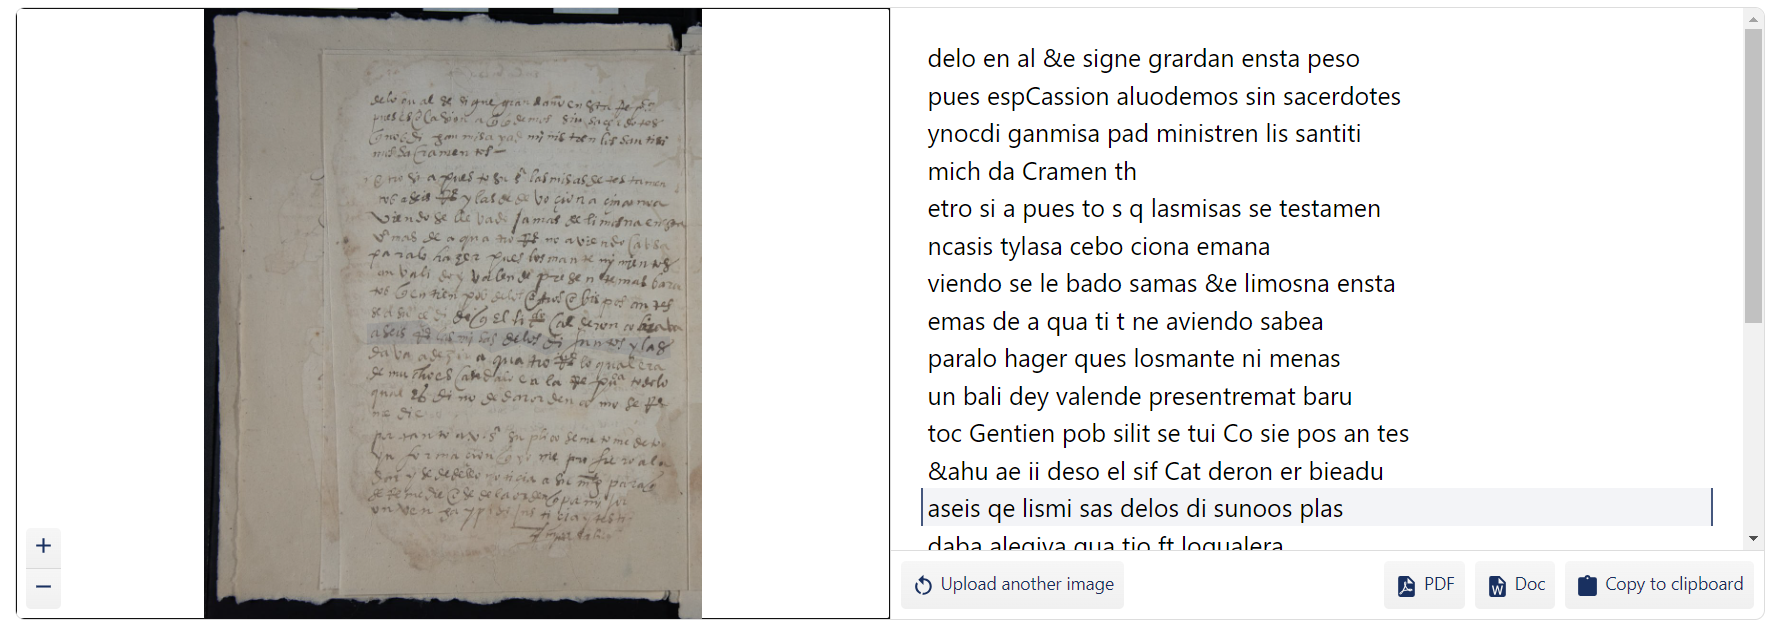
\includegraphics[width=1.0\textwidth]{transkribus} 
\end{center}

En este proyecto se afrontan dos grandes dificultades: la falta de datos para entrenar un modelo que maneje español con tipografía \textit{procesal-cortesana}, y la complejidad propia de la tarea, que normalmente requiere la atención de un especialista (tipógrafo o paleógrafo).

Ante estas circunstancias, el proyecto se orienta hacia la búsqueda exhaustiva de datos clasificados, un procesamiento minucioso de las imágenes, el uso de varios OCR y un posprocesamiento apoyado en diccionarios del idioma y un LLM.

\begin{figure}[h!]
    \centering
    \begin{tikzpicture}[node distance=2.0cm]
    
    % Bloques principales
    \node (start) [startstop] {Inicio};
    \node (clean) [process, below of=start] {Limpieza de Imágenes};
    \node (segment) [process, below of=clean] {Segmentación de Líneas};
    
    % Tres OCR, dispuestos en forma triangular debajo de "segment"
    \node (ocr1) [process, below left of=segment, xshift=-1.5cm] {OCR 1};
    \node (ocr2) [process, below of=segment, yshift=-0.5cm] {OCR 2};
    \node (ocr3) [process, below right of=segment, xshift=1.5cm] {OCR 3};
    
    % LLM debajo de los tres OCR
    \node (llm) [process, below of=ocr2, yshift=-1.0cm] {LLM correcciones};

    \node (llm2) [process, below of=llm, yshift=-1.0cm] {LLM combinaciones};
    
    % Flechas lineales
    \draw [arrow] (start) -- (clean);
    \draw [arrow] (clean) -- (segment);
    
    % Flechas desde segment a cada OCR
    \draw [arrow] (segment) -- (ocr1);
    \draw [arrow] (segment) -- (ocr2);
    \draw [arrow] (segment) -- (ocr3);
    
    % Flechas desde cada OCR hasta el LLM
    \draw [arrow] (ocr1) -- (llm);
    \draw [arrow] (ocr2) -- (llm);
    \draw [arrow] (ocr3) -- (llm);
    \draw [arrow] (llm) -- (llm2);

    \end{tikzpicture}
    \caption{Diagrama de flujo con tres OCR que convergen en el LLM y un proceso de combinaciones.}
    \label{fig:workflow}
\end{figure}

\subsection{Recursos Utilizados}

Se ha elegido Python como lenguaje principal por su facilidad de acceso a bibliotecas de procesamiento de texto e imágenes. Entre las utilizadas destacan: \texttt{Kraken}, \texttt{PIL}, \texttt{TensorFlow}, \texttt{Numpy}, \texttt{matplotlib}, \texttt{scipy}, \texttt{spaCy}, \texttt{symspellpy}, \texttt{transformers}, \texttt{cv2} y \texttt{sam2}.

El LLM utilizado es \texttt{Gemini}, principalmente por motivos económicos. Como diccionario de frecuencias se empleó \href{https://github.com/hermitdave/FrequencyWords/blob/master/content/2016/es/es_full.txt}{spanish frequency dictionary}, pues la creación de un diccionario a partir de obras antiguas resultaba muy limitada. El modelo de \texttt{spaCy} usado fue \texttt{es\_core\_news\_sm}.

\texttt{Gemini} adopta una arquitectura \textit{transformer} basada en autoatención, de forma similar a los LLM modernos. Además, se ha entrenado en un corpus mixto multilingüe que incluye español. Aunque no se especializa en español antiguo, su sólido manejo del idioma y su facilidad de uso resultaron decisivos.

Por contraste, \texttt{GPT-2} se centra mayoritariamente en inglés y requiere optimizaciones adicionales; \texttt{T5} (incluso en sus variantes \texttt{base} o \texttt{large}) demanda más recursos computacionales, encareciendo su uso continuo.

Por ello, se optó por \texttt{Gemini} como un equilibrio entre rendimiento y compatibilidad con el español, un factor esencial al manejar gran volumen de documentos y requerir un ciclo iterativo de corrección.

Para la recopilación de datos se comenzó con el \href{https://zenodo.org/records/1490009/files/Rodrigo%20corpus%201.0.0.tar.gz?download=1}{dataset de Rodrigo}, que abarca español antiguo pero tipografía gótica (no procesal-cortesana). Luego se recurrió al corpus \href{https://corpuscodea.es/}{CODEA}, con documentos anteriores a 1900 que incluyen imágenes, transcripciones paleográficas y versiones críticas. Tras filtrar por el tipo de letra requerida, el total se redujo a 546 documentos, lo cual demuestra la dificultad de obtener datos adecuados.\\

\texttt{SimpleHTR} se basa en una red neuronal recurrente (LSTM) con \textit{Connectionist Temporal Classification} (CTC) para alinear secuencias de caracteres sin segmentación estricta. Entrenado en manuscritos latinos, ofrece una estructura cercana al español antiguo.

\texttt{sinai-sam-rec-v4-best} emplea una arquitectura CRNN (red neuronal de convolución y LSTM), utilizada frecuentemente en \textit{Handwritten Text Recognition} al capturar rasgos tanto espaciales como temporales. Está optimizado para manuscritos históricos, útil ante trazos irregulares.

\texttt{McCATMuS-nfd-nofix-V1} también se basa en métodos neuronales profundos, con foco en textos históricos de variada tipografía. En particular, se ajusta a grafías antiguas y caracteres poco comunes, reduciendo la tasa de error en documentos premodernos.

\textbf{AQUÍ FALTAN AGREGAR RESULTADOS} (comparación de cada OCR)\\

\section{Resultados}
\subsection{Logros Principales}

En la primera etapa se logra una mejora considerable de las imágenes, aplicando un pipeline de limpieza que las convierte a escala de grises e incluye varias técnicas de filtrado (filtro gaussiano para reducir ruido, ecualización de histograma para mejorar contraste, y operaciones morfológicas de erosión y dilatación para resaltar los trazos). Finalmente, se emplea la binarización de \texttt{Kraken}, con redes neuronales profundas y binarización adaptativa entrenada en documentos históricos. En la figura \ref{fig:tresfotosmodelo} se observa la evolución desde la imagen original hasta la binarizada.

Para tratar las manchas producidas por la antigüedad (tonos amarillos), se implementa un conversor personalizado a escala de grises que pondera \textit{r} y \textit{g} de forma distinta a la habitual, atenuando así el efecto amarillo.

\begin{figure}[h] 
\centering 
\begin{minipage}{1.0\textwidth} 
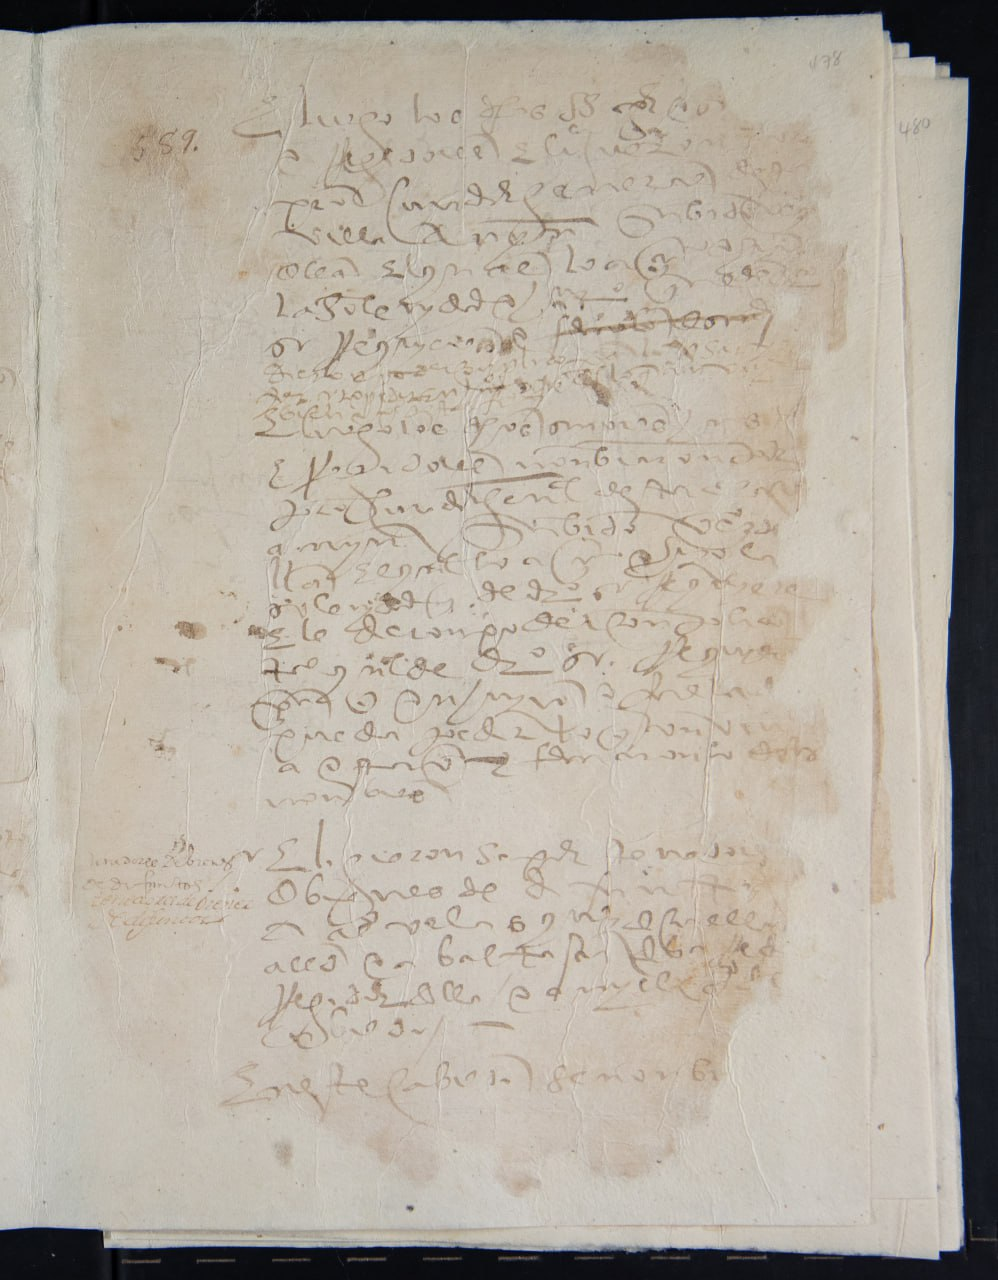
\includegraphics[width=0.32\textwidth]{original.jpg} 
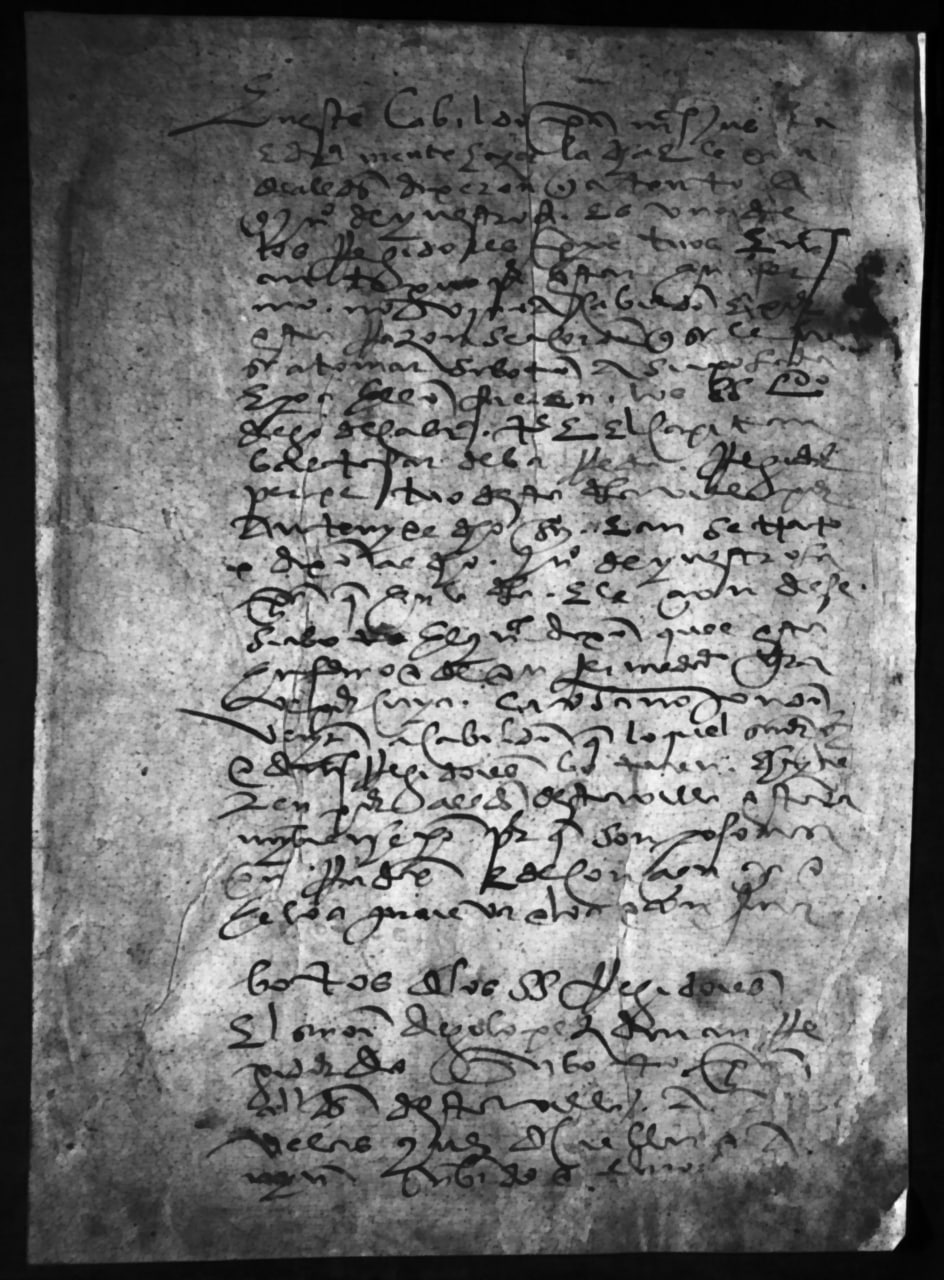
\includegraphics[width=0.32\textwidth]{morph.jpg} 
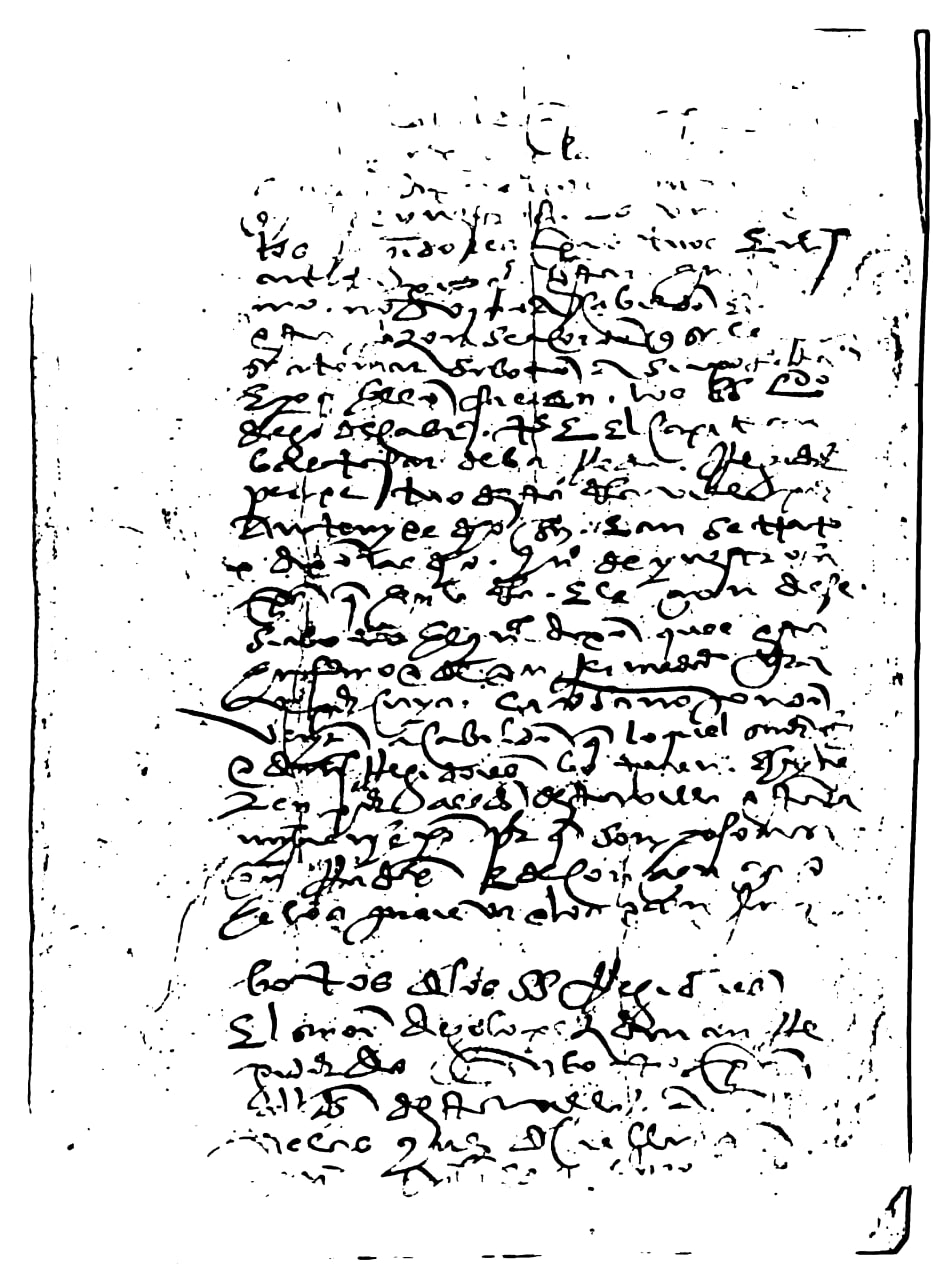
\includegraphics[width=0.32\textwidth]{kraken.jpg} 
\caption{Original, en escala de grises con letra reforzada, e imagen binarizada.} 
\label{fig:tresfotosmodelo} 
\end{minipage} 
\end{figure}

También se evalúan algoritmos de detección de bordes como \textit{sobel}, \textit{Canny} y \textit{laplaciano}. El último no funciona bien por su sensibilidad a cambios drásticos pixel a pixel (papel vs. tinta). Sobel y Canny muestran algunos buenos resultados en ciertos documentos, como se aprecia en la figura \ref{fig:tresfotos}, pero no de modo uniforme.

\begin{figure}[h] 
\centering 
\begin{minipage}{1.0\textwidth} 
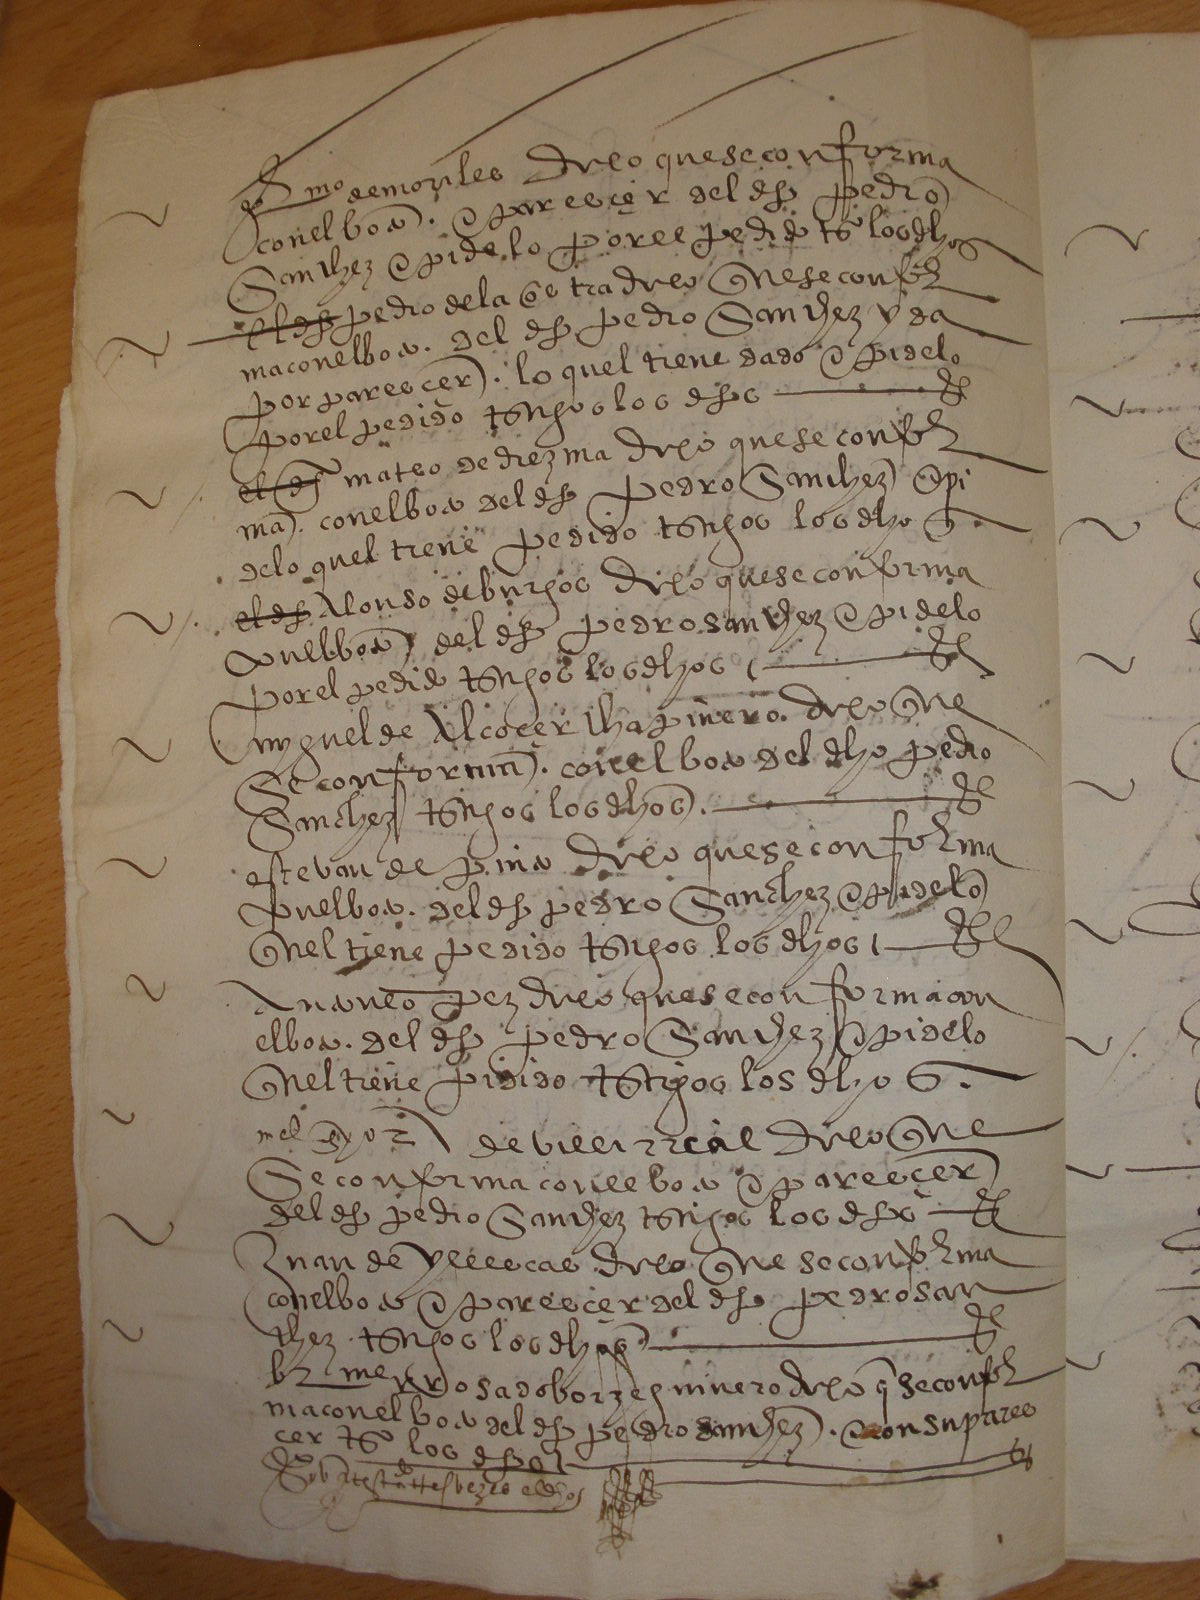
\includegraphics[width=0.32\textwidth]{CODEA-0205_2v.jpg} 
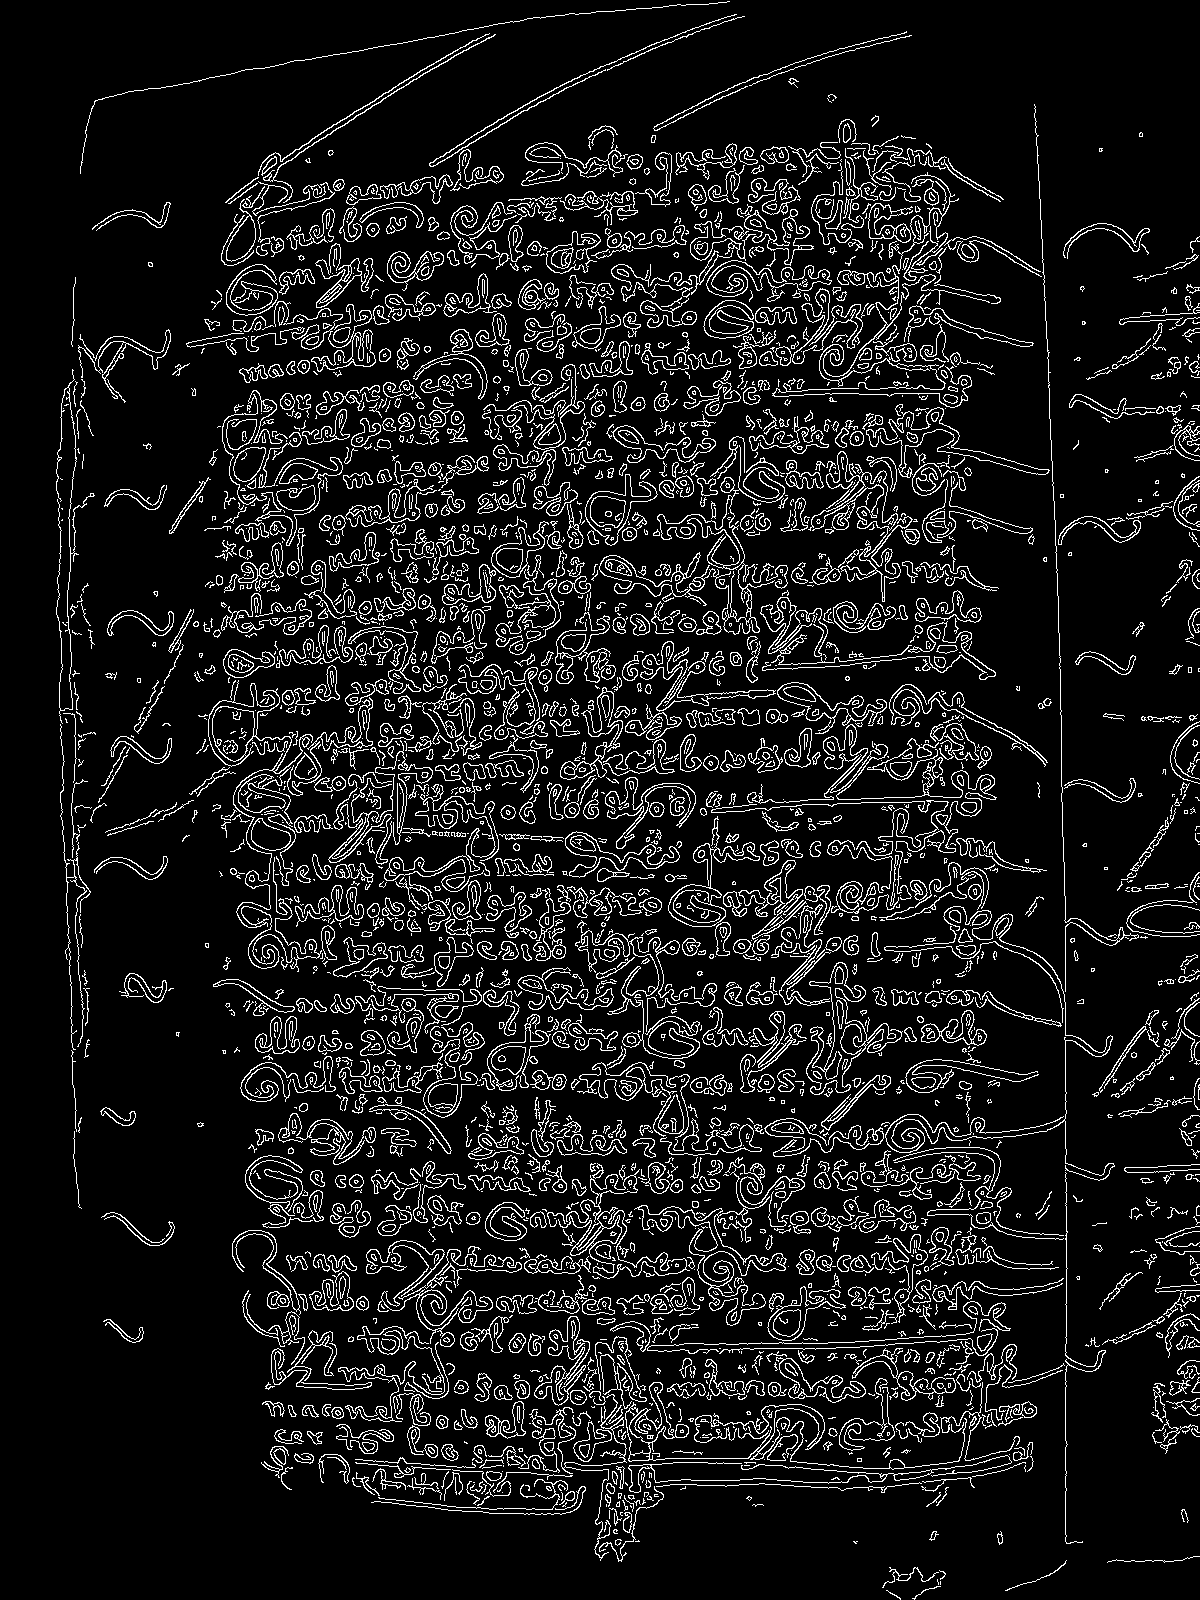
\includegraphics[width=0.32\textwidth]{canny_image_aftergauss_eq2.png} 
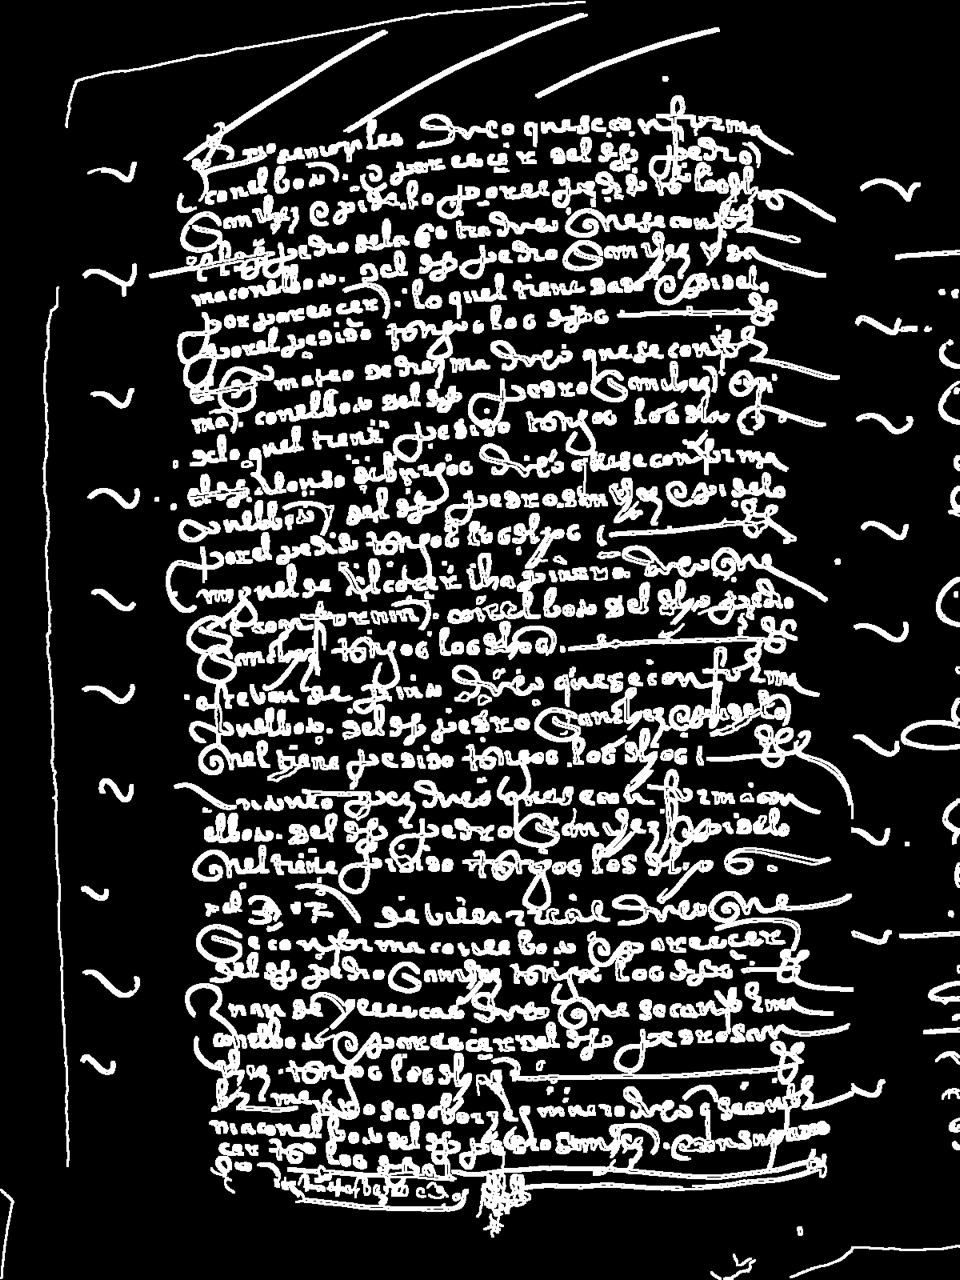
\includegraphics[width=0.32\textwidth]{photo_2025-01-27_21-34-01.jpg} 
\caption{Original, detección de bordes y operaciones morfológicas (de izquierda a derecha).} 
\label{fig:tresfotos} 
\end{minipage} 
\end{figure}

También se prueba el filtrado mediano para reducir el ruido “sal y pimienta” y el filtrado bilateral, sin mejoras significativas. La binarización mediante un umbral fijo no detecta bien la letra en zonas de sombra, y la binarización adaptativa convencional recupera demasiado ruido.\\

Tras la binarización, las imágenes pasan por dos procesos de segmentación: uno interno de \texttt{Kraken} y otro basado en proyección de histogramas. El primero ofrece resultados superiores. Para segmentaciones manuales se investiga \texttt{SAM2}, sin lograr automatización completa. Dicha herramienta es efectiva con líneas rectas, algo que no se cumple en manuscritos antiguos.\\

Finalmente, la imagen segmentada se procesa con tres OCR distintos: \texttt{SimpleHTR}, \texttt{sinai-sam-rec-v4-best} y \texttt{McCATMuS-nfd-nofix-V1}. Los dos últimos aprovechan \texttt{Kraken}, mientras que \texttt{SimpleHTR} requiere una segmentación previa en líneas.

\subsection{Posprocesamiento y Combinación}

Después de extraer el texto con los distintos OCR, se procede a un posprocesamiento para mejorar la fidelidad de las transcripciones. Inspirándose en el dataset de CODEA, se adopta una transcripción crítica de los documentos. Dada la complejidad de los manuscritos y los errores de OCR, se implementa un pipeline que corrige errores ortográficos y refina la coherencia.

En primer lugar, se usa \texttt{spaCy} para segmentar el texto en \textit{tokens}, aislando palabras y símbolos no alfabéticos. Cada palabra se corrige con \texttt{SymSpell}, que se apoya en un diccionario de frecuencias para separar palabras unidas y reponer grafías correctas. Luego, un modelo generativo (\texttt{Gemini}) refina la semántica y el estilo, ayudando a mantener un tono cercano al español antiguo.

\textbf{Combinación de OCR con el LLM.}  
Para unificar las salidas de los tres OCR (\texttt{SimpleHTR}, \texttt{sinai-sam-rec-v4-best} y \texttt{McCATMuS-nfd-nofix-V1}), se emplea \texttt{Gemini} con un enfoque de “prompt colaborativo”. Este recibe:

\begin{itemize}
\item Texto A: salida del OCR 1  
\item Texto B: salida del OCR 2  
\item Texto C: salida del OCR 3
\end{itemize}

Se le indica que compare las tres versiones, identifique coincidencias y divergencias, corrija inconsistencias ortográficas o gramaticales, y produzca una transcripción unificada fiel al original histórico. Gracias a la base en español y la capacidad generativa, \texttt{Gemini} pondera cada fragmento, compensando errores de un OCR con aciertos de otro.

Por ejemplo:

\begin{enumerate}
    \item Essta es una prueva de ectraccion de teexto. Connoscida cosa sea a todos los queesta carta uieren como yo don Fferrando por la gracia de dios hey de Castiella
    \item Esta es una prueba de extracción de texto. Conocida cosa sea a todos los que esta carta vieren como yo don Fferrando por la gracia de Dios hay de Castilla
    \item Esta es una prueba de extracción de texto. Conocida cosa sea a todos aquellos que esta carta vieran, como yo, don Fernando, por la gracia de Dios, rey de Castilla.
\end{enumerate}

\subsection{Desafíos Superados}

Uno de los principales retos se observa en la segmentación, que precisa ajustar parámetros para optimizar los siguientes pasos. 

Además, la conservación del español antiguo complica el posprocesamiento. Al no existir un diccionario de frecuencias específico, se recurre a un LLM que, si bien no es perfecto, ofrece una aproximación plausible. Se evalúan \texttt{GPT-2}, \texttt{google/mt5-small} y \texttt{flax-community/spanish-t5-small}, pero fracasan por limitaciones de recursos o mala adaptación al dominio. Finalmente, \texttt{Gemini} cumple con la exigencia, equilibrando precisión y costo de uso.

\section{Conclusiones}
\subsection{Impacto del Proyecto}

Este proyecto se concibe para la transcripción de documentos históricos resguardados en la Oficina del Historiador. Inicialmente se cuenta con un tomo digitalizado, y a medida que se digitalicen los siguientes, se podrán aplicar directamente estas técnicas de transcripción y análisis. Asimismo, los resultados pueden servir de base para productos reutilizables, como herramientas que busquen entidades o información valiosa en estos manuscritos.

\subsection{Recomendaciones para Futuras Implementaciones}

Se sugiere explorar el uso de \textit{DBSCAN} para la segmentación de líneas en manuscritos curvos e irregulares, propios de la tipografía \textit{procesal-cortesana}. También se recomienda entrenar o afinar (\textit{fine-tuning}) \texttt{SimpleHTR} y el modelo generativo para mejorar la precisión en español antiguo. Por último, \texttt{GPT-2} podría reutilizarse entrenándose específicamente en este dominio, lo que potencialmente derivaría en buenos resultados.

\bibliographystyle{plain} 
\bibliography{referencias}

\begin{thebibliography}{9}

    \bibitem{Avila2020corpus}
    Vicente Marcet Rodriguez,
    \textit{El copus de documentos de \'Avila del Hispanic Museum and Library (siglos XV y XVI). Descripci\'on y an\'alisis paleogr\'afico y gr\'afico-fonol\'ogico.}

    \bibitem{granet2018transfer}
    A. Granet, E. Morin, H. Mouchère, S. Quiniou, y C. Viard-Gaudin, 
    \textit{Transfer Learning for Handwriting Recognition on Historical Documents}, 
    ICPRAM, 2018.
    
    \bibitem{torres2025htr}
    S. Torres Aguilar, 
    \textit{Handwritten Text Recognition for Historical Documents using Visual Language Models and GANs}, 
    ArXiv, 2025.
    
    \bibitem{granell2018transcription}
    E. Granell, E. Chammas, L. Likforman-Sulem, C. D. Martínez-Hinarejos, C. Mokbel, y B. I. Cîrstea, 
    \textit{Transcription of Spanish Historical Handwritten Documents with Deep Neural Networks}, 
    Journal of Imaging, vol. 4, no. 15, 2018.
    
    \bibitem{survey_post_ocr}
    THI TUYET HAI NGUYEN, ADAM JATOWT, MICKAEL COUSTATY and ANTOINE DOUCET,
    \textit{Survey of Post-OCR Processing Approaches}, 
    2025.

    \bibitem{LightweightOCR}
    Yuning Du, Chenxia Li, Ruoyu Guo, Xiaoting Yin, Weiwei Liu,
    Jun Zhou, Yifan Bai, Zilin Yu, Yehua Yang, Qingqing Dang, Haoshuang Wang,
    \textit{PP-OCR: A Practical Ultra Lightweight OCR System}
    
    \bibitem{IJARSCT2023extraction}
    Prof. Anuradha Thorat, Mayur Zagade, Shivani More, Manish Pasalkar, Anand Narute,
    \textit{Research Paper on Text Extraction using OCR}, 
    IJARSCT, Volume 3, Issue 14, May 2023

    \bibitem{IJIREM2022extraction}
    Ojas Kumar Barawal, and Dr Yojna Arora,
    \textit{Text Extraction from Image}, 
    IJIREM, Volume 9, Issue 3, May 2022

\end{thebibliography}

\end{document}
